\chapter{Completed Work}\label{sec:completed_work}

\section{Transfemoral Prosthesis Design}\label{sec:completed_design}
\begin{marginfigure}[1.25in]
    \centering
    \includegraphics[width=\linewidth]{prosthesis_render_annotated}
    \caption{Render of proposed powered knee and ankle prosthesis design. The
    prosthesis includes series elastic actuators to enable accurate torque
    control and a unidirectional parallel ankle spring to offset the required
    angle torque.}\label{fig:prosthesis_render_annotated}
\end{marginfigure} 

\newthought{To test our proposed Neuromuscular control approach}, and its
ability to help subjects maintain or recover their balance, we build a custom
transfemoral prosthesis capable of reproducing dynamic locomotion tasks. The
proposed design, shown in \cref{fig:prosthesis_render_annotated}, uses brushless
electric motors coupled to harmonic drive gear sets to drive both the knee and
ankle joints.  Additionally, the joints employ series elastic actuation to
enable accurate torque control and to protect the prosthesis' gear sets from
sudden impacts.  The design also features a unidirectional parallel spring in
the ankle that partly offsets the torque demands on the ankle motor.  We design
both joints to meet the demands of dynamic locomotion tasks such as running and
trip recovery.

The overall design concept sits in a niche between low powered prostheses
designed with commercial applicability in mind
\citep{sup2007design,sup2009preliminary,lawson2014robotic,rouse2015design,
martinez2011antagonistic} which feature onboard actuation and power sources, and
high-powered tethered systems \citep{caputo2013experimental,
caputo2015informing} with off-board actuation designed exclusively for use in
lab environment. Our design features onboard actuators that are more powerful
than those used in standalone devices, but less capable than those employed in
tethered devices. To ensure a reasonable overall weight the device's batteries,
motor drivers, and computers are off-board. With this design, we expect to be
able to test control ideas without encountering hardware performance limitations
as with a tethered device. At the same time the device is capable of functioning
outside of the lab environment like a standalone prosthesis. 

\begin{table}
    \centering
    \begin{tabular}{lcc}
        \toprule
        Specification         & Desired Value & Achieved Value \\
        \midrule                  
        Maximum Knee Torque   & $\unit[160]{N \cdot m}$ 
            & $\unit[170]{N \cdot m}$   \\
        Maximum Knee Speed    & \unitfrac[1.80]{rev}{s} 
            & \unitfrac[1.93]{rev}{sec} \\
        Knee Torque Bandwidth & \unit[4]{Hz} & \unit[11.7]{Hz} \\
        Maximum Ankle Torque  & $\unit[200]{N \cdot m}$ 
            & $\unit[170 \ (+120^*)]{N \cdot m}$ \\
        Maximum Ankle Speed   & \unitfrac[1.14]{rev}{s} 
            & \unitfrac[1.22]{rev}{s} \\
        Ankle Torque Bandwidth & \unit[3.5]{Hz} & \unit[5.9]{Hz}\\
        Weight                & \unit[6.8]{kg} & \unit[5.9]{kg} \\
        Minimum Height        & \unit[42.5]{cm} & \unit[42]{cm} \\
        \bottomrule
    \end{tabular}
    \caption{Designed and achieved design specifications. ($^*$Maximum total
    ankle torque is $\unit[290]{N \cdot m}$ achieved at \unit[10]{degrees} of
    dorsiflexion.)}\label{tab:pros_requirements}
\end{table}

\Cref{tab:pros_requirements} shows the desired design specifications for the
transfemoral prosthesis and the values achieved by the final design. To obtain
these design specifications we examined a number of studies that elicited trip
responses.

We specify desired joint torque and speed values to meet the requirements of
demanding tasks such as running. The maximum knee torque specification comes
from the findings of \citet{whitley2008maximum}, who tested the joint torques
used during recovery from a simulated fall. The maximum knee speed requirement
comes from \citet{grabiner1993kinematics}, who tested subjects' responses to
simulated trips induced by unseen obstacles on a walkway. We obtain the maximum
ankle torque requirement from \citet{pijnappels2005early}, who tripped subjects
using a obstacles that could suddenly emerge through the floor. The maximum
ankle speed requirement comes from the running data of
\citet{novacheck1998biomechanics}. We set to the minimum height specification,
measured between the center of the knee and bottom of the foot, to accommodate
the $10^\tn{th}$ percentile female \citep{gordon1988anthropometric}.  Finally,
the required weight corresponds to the mean leg weight of a $50^\tn{th}$
percentile male \citep{winter2009biomechanics}.

\subsection{Knee Joint}
\begin{marginfigure}[2in]
    \centering 
    \includegraphics[width=\linewidth]{knee_motor_torque}
    \caption{Knee motor torque required for
    running}\label{fig:knee_motor_torque}
\end{marginfigure}
In addition to achieving the maximum speeds and torques found in
\cref{tab:pros_requirements}, we design the knee joint so that it can reproduce
the torque and speed required for a \unit[80]{kg} person to run at
\unitfrac[3.2]{m}{s} as measured by \citet{novacheck1998biomechanics}. To
reproduce this trajectory in the knee joint, we utilize a RoboDrive ILM
$85\times13$ HS-SP motor coupled to a Harmonic Drive Gear set with a 50:1
reduction (CSG--25--50). \Cref{fig:knee_motor_torque} shows the motor torque
and speed required to reproduce a running trajectory assuming a gear
efficiency of $75\%$. In this plot, we see that the running trajectory lies
within the speed-dependent torque limit of the motor. Moreover, the root mean
squared torque of this trajectory $(\unit[1.46]{N \cdot m})$ exceeds the torque
rating of the motor $(\unit[1.43]{N \cdot m})$ by just $2\%$. Therefore, the
knee joint should be able to provide the necessary torque to enable running for
a short amount of time, or continuously for lighter subjects or at a slightly
reduced speed.

\begin{figure*}[t]
    \centering 
    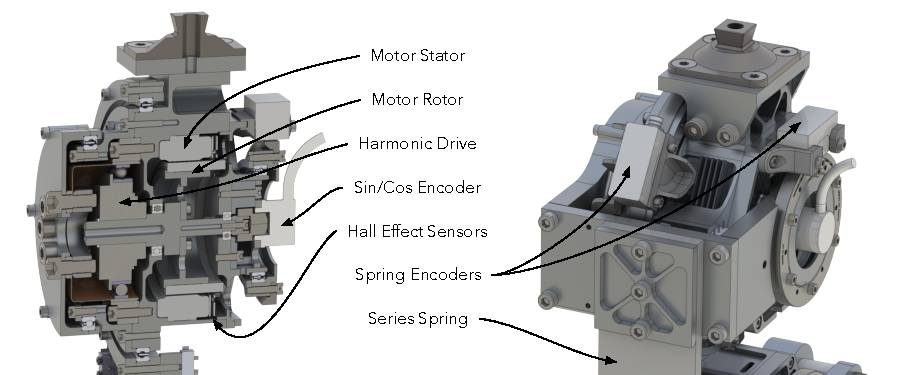
\includegraphics[width=\linewidth]{knee_design}
    \caption{Internal and external design of the knee 
    joint.}\label{fig:knee_design}
\end{figure*}
\Cref{fig:knee_design} shows the internal and external design of the knee joint.
The primary component in the knee joint is the stator housing. On top of the
housing is a standard pyramid adaptor that allows the prosthesis to connect to
amputee's sockets. Within the stator housing, lies the brushless motor stator,
rotor, and harmonic drive gear set. We sense absolute rotor angle for
commutation of the brushless motor via hall effect sensors and a magnetic
complementary sin/cos encoder. To incorporate series elasticity, we take
inspiration from the design of the bipedal robot Atrias
\citep{grimes2013atrias}, which uses fiberglass series leaf springs. In our
design, the output of the gear set drives the proximal end of a fiberglass leaf
spring in series with the shank. Two Renishaw Resolute absolute encoders measure
the deflection of this spring to enable torque control.

\begin{marginfigure}[2.5in]
    \centering 
    \includegraphics[width=\linewidth]{knee_impact_sim}
    \caption{Impact simulation we used to determine appropriate series spring
    stiffness.}\label{fig:knee_impact_sim}
\end{marginfigure}
In addition to allowing for accurate torque control, as shown by
\citet{au2007biomechanical,au2008powered}, the series elasticity also plays a
crucial role in protecting fragile gear components from impact loads. To choose
the spring stiffness for the knee joint, we simulate the prosthesis impacting a
rigid wall with the foot during swing. To do this, we construct a model of the
prosthesis in Matlab Simulink Simscape Multibody that includes the
series elasticity, gear dynamics, and motor electrical dynamics.
\Cref{fig:knee_impact_sim} shows the simulation environment. The prosthesis is
attached to the distal end of a thigh segment with a fixed hip position. We
control the hip via the ideal swing leg control outlined in
\cref{sec:neuro_ideal_swing} (\cref{eq:hipfeedback}) and consider the case where
the external voltage applied to the motor is zero. This simulation suggests that
a spring stiffness under $\unitfrac[2300]{N \cdot m}{rad}$ will ensure that the
peak impact torque remains lower than the peak allowable impact torque of the
Harmonic Drive of $\unit[242]{N \cdot m}$.

We can also estimate the torque bandwidth of the actuator by analyzing the SEA
dynamics for the system depicted in \cref{fig:sea_diagram}. Assuming the load
is fixed, the transfer function between the motor and load torques is given by
\begin{align}
    \frac{\tau_l}{\tau_m} = \frac{\nicefrac{k}{J_m}}{s^2 + \nicefrac{k}{J_m}}
\end{align}
where $\tau_l$ and $\tau_m$ are the load torque and post-gearbox motor torque
respectively. $J_m$ is the sum of the reflected motor rotor inertia and inertia
of components that form the motor-side attachment of the spring, which has
stiffness $k$. From this equation we calculate the bandwidth of the system
to be
\begin{align}
    f_{3 dB} = \frac{\sqrt{\nicefrac{k}{J_m}}}{2 \pi}.
\end{align}
For a spring stiffness of $\unitfrac[2300]{N \cdot m}{rad}$ we estimate the
torque bandwidth is \unit[11.7]{Hz}. This value exceeds the required torque
bandwidth of \unit[4]{Hz} given by \citet{sergi2012design} (obtained by
analyzing the torque data for walking reported by
\citet{winter2009biomechanics}). However, it should be noted that this is a very
crude estimate of bandwidth. On the one hand, it may underestimate the true
value, as it assumes that to achieve a desired output torque, the motor control
applies the same torque to the motor side of the spring. In practice, a
closed-loop torque control can transiently apply much larger torques to the
motor side in order to achieve faster convergence to a desired steady-state
output torque. On the other hand, this value may also underestimate the true
bandwidth, as it does not consider the motor's voltage-current dynamics or gear
friction.

\subsection{Ankle Joint}
In the ankle joint we utilize a RoboDrive ILM $70\times10$ HS-SP motor coupled
to a Harmonic Drive Gear set with a 100:1 reduction (CSG--20--100). As with the
knee joint, we design the ankle joint to satisfy the requirements listed in
\cref{tab:pros_requirements}. Specifically, for the ankle joint we pay
considerable attention to the tripping condition described by
\citet{pijnappels2005early}, in which the ankle generates a peak torque of
$\unit[202]{N \cdot m}$. 

To avoid using a large and heavy motor to achieve this peak torque, we take
inspiration from previous prosthetic ankle designs that employ a unidirectional
parallel spring in the ankle joint that performs the conservative portion of the
ankle's torque versus angle trajectory during normal walking
\citep{au2007biomechanical,au2008powered,sup2009preliminary,lawson2014robotic}.
The parallel spring offsets the required motor torque, as the actuator only
needs to provide the difference between the desired torque and the torque
provided by the parallel spring. \Cref{fig:ankle_torque_vs_angle_ups} shows the
torque versus angle curve during level ground walking
(\citet{winter2009biomechanics}, scaled to \unit[80]{kg} person). In green we
show the torque generated by a $\unitfrac[700]{N \cdot m}{rad}$ parallel spring
optimized to minimize the root-mean-squared motor torque for this trajectory.
From this plot, we see that with the parallel spring, the peak torque is lower
than the repeated peak torque limit of the Harmonic Drive Gear set.

\begin{marginfigure}[-0in]
    \centering 
    \includegraphics[width=\linewidth]{ankle_torque_vs_angle_ups}
    \caption{Ankle torque vs angle curve during steady, level-ground walking
    (blue) (\citet{winter2009biomechanics} scaled to \unit[80]{kg} person). A
    unidirectional parallel spring can provide a portion of this torque (green)
    and reduces the required actuator torque (purple) to lie under repeated
    torque limit of the Harmonic Drive Gear set (orange).
    }\label{fig:ankle_torque_vs_angle_ups}
\end{marginfigure}

The tripping data obtained by \citet{pijnappels2005early} shows that the ankle
kinematics during trip recovery are similar to those seen during normal walking.
Therefore, the parallel spring, should be able to contribute torque during the
tripping case as well. To confirm this, \cref{fig:ankle_motor_torque_tripping}
shows the motor torque required for trip recovery (obtained by scaling walking
torque data from \citet{winter2009biomechanics} to have a peak torque of
$\unit[202]{N \cdot m})$ We see that the inclusion of the parallel spring allows
the prosthesis to produce enough net torque to reproduce the trip recovery
trajectory without exceeding the torque limit of the motor. 
\begin{figure}[b]
    \centering 
    \includegraphics[height=2in]{ankle_motor_torque_tripping}
    \caption{Ankle motor torque required to take the trip recovery action
    observed by \citet{pijnappels2005early} (blue, trajectory obtained by
    scaling walking data from \citet{winter2009biomechanics} to a peak torque of
    $\unit[202]{N \cdot m}$, $75\%$ gear efficiency assumed). Using a parallel
    spring allows the motor to produce the required torque (green) while
    remaining within it's torque limit (purple).
    }\label{fig:ankle_motor_torque_tripping}
\end{figure}

Finally, \cref{fig:ankle_motor_torque_running} shows the torque and speed
required of the motor for running \citep{novacheck1998biomechanics}. In this
case, we use an ankle parallel stiffness of $\unitfrac[267]{N \cdot m}{rad}$.
From this plot, we see that this combination of ankle motor and spring is nearly
sufficient for running. Increasing the voltage of the prosthesis from
\unit[48]{V} to \unit[60]{V} or decreasing the gear ratio from 100:1 to 80:1
will allow the torque trajectory to fit completely within the motor limits. 
\begin{marginfigure}[-0in]
    \centering 
    \includegraphics[width=\linewidth]{ankle_motor_torque_running}
    \caption{Ankle motor torque required to reproduce the running trajectory
    recorded by \citet{novacheck1998biomechanics} assuming a parallel spring
    stiffness of $\unitfrac[267]{N \cdot m}{rad}$ and a gear efficiency of
    $75\%$.
    }\label{fig:ankle_motor_torque_running}
\end{marginfigure}

\Cref{fig:ankle_design} shows an internal view of the ankle actuator and
external views of the actuator and foot mechanism. In the ankle design, the
output of the actuator actuates the foot through a four-bar mechanism. The
actuator pulls or pushes on the proximal end of a length-adjustable tendon. The
distal end of the tendon attaches to one end of a fiberglass series elastic leaf
spring that is also connected to the foot. By measuring the angles of the ankle
actuator output and the ankle joint and using the equations of the four-bar
mechanism's kinematics, we can calculate the deflection of the leaf spring and
thus the torque applied to the ankle.
\begin{figure*}[b!]
    \centering 
    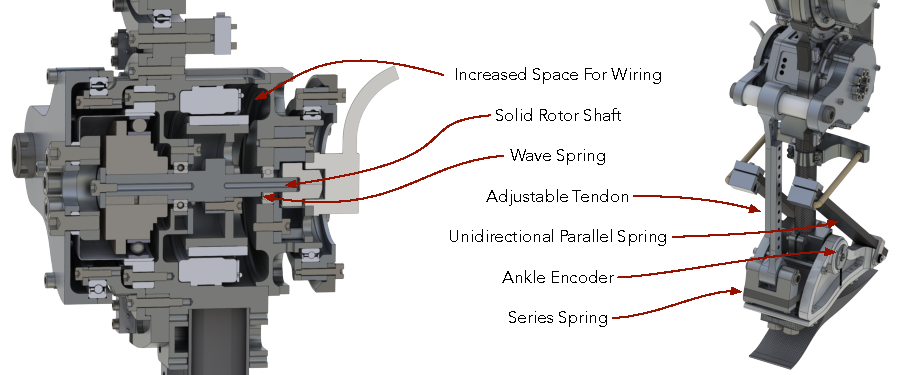
\includegraphics[width=\linewidth]{ankle_design}
    \caption{Internal and external design of the ankle 
    joint.}\label{fig:ankle_design}
\end{figure*}

The design of the ankle actuator represents a second iteration of the knee
actuator design and features two main improvements.  First, it has increased
space on the side of the motor for cable routing. Second, the ankle actuator has
a solid rotor shaft. In contrast, the knee actuator's shaft is comprised of two
parts: one that held the motor rotor and transferred power through the gear set,
and another that held the sin/cos encoder's magnetic shaft component. In
practice, these two components proved difficult to align, causing degraded
performance of the sin/cos encoder. The ankle actuator's solid shaft ensures the
encoder magnet stays aligned with the read head.

\begin{marginfigure}[-0.0in]
    \centering 
    \includegraphics[height=2in]{ankle_impact_sim}
    \caption{Impact simulation we used to determine appropriate series spring
    stiffness.}\label{fig:ankle_impact_sim}
\end{marginfigure}
As we did for the knee series spring, we again determine an acceptable ankle
spring stiffness by performing an impact simulation. For the ankle, we simulate
an \unit[80]{kg} person stepping on the prosthesis when the motor driver
provides the ankle motor with zero applied voltage. \Cref{fig:ankle_impact_sim}
shows the simulation environment. From this simulation we find that a spring
stiffness of about $\unitfrac[1000]{N \cdot m}{rad}$ should sufficiently protect
the ankle gear set from impacts. This estimate is likely softer than necessary
due to the additional series compliance in the amputee's socket and the
composite foot that are not included in the simulation.
Repeating the bandwidth calculation we performed for the knee spring, we
estimate the ankle bandwidth may be around \unit[5.9]{Hz}. This value exceeds
the required torque bandwidth of \unit[3.5]{Hz} given by \citet{au2008powered}
(obtained by analyzing the torque data for walking reported by
\citet{winter2009biomechanics}).

\section{Experiments on Powered Knee/Passive Ankle
Prosthesis}\label{sec:complete_exp} 

\emph{Material in this section based partially on
\citet{thatte2016toward}\cite{thatte2016toward}}
\linebreak

Towards a full realization and study on amputee subjects, we present a partial
implementation and evaluation of the control on the current prosthesis prototype
worn by a non-amputee user. \Cref{fig:test_bed_annotation} shows an able-bodied
user wearing our current prosthesis prototype. The current prosthesis prototype
has an active knee SEA unit and an unpowered, spring-loaded, ankle.  We connect
the prosthesis to a knee crutch (iWalk 2.0 Hands Free Crutch) in order to allow
a non-amputee experimenter to test the control. Additionally, the experimenter
wears a lift shoe to compensate for the added thigh length of the knee crutch
and prosthesis.
\begin{figure}
    \centering 
    \includegraphics[height=3in]{test_bed_annotation}
    \caption{A non-amputee experimenter tests the prosthesis using an iWalk
    Crutch as a knee adaptor. The experimenter wears a lift shoe on the
    contralateral leg to compensate for the added thigh length of the prosthesis
    and knee adaptor.
    }\label{fig:test_bed_annotation}
\end{figure}

To control the prosthesis knee, we use Simulink Real-Time (Mathworks, USA),
which samples all sensors (joint encoders, IMU on thigh, force sensors in foot),
runs a velocity-based SEA control \citep{schepelmann2012development}, and sends
commands to the motor controller at a rate of 1kHz. Given a desired torque,
$\tau_\tn{d}$, and a measured torque error, $\tau_\tn{e}$, the commanded motor
velocity is given by
\begin{align}
    \omega_\tn{m} = \frac{1}{k} \frac{\tn{d} \tau_\tn{d}}{\tn{d} t} 
        + (1 + k_\tn{d})\omega_\tn{l} + \func{PD}{\tau_\tn{e}},
    \label{eq:velocity_based_sea}
\end{align}
where $\omega_\tn{l}$ is the velocity of the load-side of the series spring (the
shank), $k_\tn{d}>0$ compensates for damping in the knee bearing, and
$\func{PD}{\cdot}$ is a proportional-derivative feedback term. 

The behavior control of the knee is a hybrid model that combines the
Neuromuscular Stance control described in \cref{sec:neuro_stance_reflexes} with
the idealized swing control outlined in \cref{sec:neuro_ideal_swing}. The
missing ankle actuation in the current prosthesis prototype restricts the
neuromuscular stance control to those muscles that span the knee: the vastus,
hamstring, and gastrocnemius. The hamstring and vastus are stimulated according
to \cref{eq:ham_stim_full,eq:vas_stim_full} respectively.  Similarly, the
gastrocnemius is stimulated by positive force feedback. (The torso balance
contribution of the complete hamstring stimulation, \cref{eq:ham_stim_full}, is
neglected.) The realtime software executes the hybrid neuromuscular behavior
control at a rate of 5kHz, ensuring that the integration (ode1) of the simulated
muscle dynamics remains stable. During swing, we only use the knee portion of
the swing control given by \crefrange{eq:flexphase}{eq:extend}. In late swing,
the control transitions between the two phases in proportion to the measured
ground reaction force (\cref{eq:stance_grf_trans,eq:swing_grf_trans}).

% Generation of normal stance behavior
\subsection{Slow Walking Behavior}\label{sec:completed_knee_exp_walk}
We first test if the prosthesis control can reproduce normal stance and swing
behavior of the lower limb in steady-state walking. For this purpose, we capture
joint kinematics and kinetics as well as the virtual muscle activations of the
prosthesis control while an experimenter walks for ten trials with the crutch
and prosthesis system on a treadmill. Because the fit of the crutch to the
experimenter's leg is not very tight, we limit the walking speed to
\unitfrac[0.5]{m}{s} and the experimenter holds onto handrails for safety
(\cref{fig:test_bed_annotation}).
\begin{figure}[t]
    \centering
    \includegraphics[width = 3in]{pros_gait_data}
    \caption{Prosthesis behavior at walking speed of 0.5 m/s. Shown are the hip
    and knee trajectories, the knee controller torque, and the activations of
    the vastus, hamstring, and gastrocnemius muscles generated by the
    prosthesis control in the testbed. Solid black lines show averaged data  of
    ten trials with the individual trials depicted in gray. Dashed lines show
    corresponding data from human walking at preferred speed (joint angles and
    knee torque: \citet{winter2009biomechanics}, muscle surface
    electromyograms: \citet{perry2010gait}). Solid and dashed vertical lines
    indicate median toe off times for the prosthesis and human data
    respectively.
    }\label{fig:pros_gait_data}
\end{figure}

The control generates steady-state prosthesis behavior that qualitatively
reproduces human leg behavior in walking. \Cref{fig:pros_gait_data} compares the
observed prosthesis leg behavior (solid lines) to corresponding human data at
preferred walking speed (dashed lines, adapted from
\citet{winter2009biomechanics,perry2010gait}). The hip and knee kinematics match
overall, although later transitions from stance to swing are observed in both
joints ($\theta_\tn{h}$ and $\theta_\tn{k}$) and the prosthesis knee flexes less
in stance ($\theta_k$). The knee torque follows trends similar to human data,
but the peak flexion and extension torques in the early stance phase are
diminished ($\tau_\tn{k}$). These lower peaks are caused by reduced activations
of the virtual vastus and hamstring muscles (VAS and HAM) in this phase, a clear
difference to these muscles' activation in humans, in which bursts of activity
at heel strike are followed by relative silence. Finally, the activity of the
virtual gastrocnemius muscle (GAS) bears strong similarity the activity of this
muscle in human walking.

To some extent, limitations of our current experimental testbed may
account for observed discrepancies. The imposed slow walking speed of 0.5 m/s
required less energy absorption in early stance than at normal walking speed.
Moreover, the experimenter held onto the handrails to assist with lateral
balance, which may have channeled some impact energy through the arms. In
addition, the hybrid nature of the proposed control prevents the virtual
muscles from activating in swing, which is the case in humans
(\cref{fig:pros_gait_data}, VAS and HAM activities from 80\% to 100\% of gait
cycle), and would alter the response of the virtual muscles at heel strike.
Finally, the lack of an active ankle and its control in the current prosthesis
prototype further limits how closely the leg behaviors can match.

% Response to Swing Leg Tripping
\subsection{Response to Swing Leg Tripping}\label{sec:completed_exp_swing_trip}
 

In a second set of experiments, we evaluate the response of the prosthesis
controller to trip disturbances. We apply disturbances during treadmill walking
by commanding flexion knee torques to the prosthesis in addition to its
swing-leg control torque. The added torque simulates an obstacle encounter
modeled in the same way as the stopping torque of the swing leg control,
\cref{eq:stop}, with $\alpha_{thr}$ replaced by a disturbance leg angle. The
foot can pass the simulated obstacle if the leg length contracts beyond a
threshold of \unit[94]{cm}. For an early-, mid-, or late-swing encounter, the
disturbance angle is set to 110, 95, or \unit[80]{degrees}, respectively. In
addition, anticipation of the trip by the experimenter is prevented by applying
the disturbance only with a probability of 25\%.

\begin{marginfigure}[1in]
    \centering
    \includegraphics[width = \linewidth]{impulse_hardware_annotated.pdf}
    \caption{Response to simulated tripping disturbance. (A) Undisturbed ankle
    trajectory calculated from hip and knee angles assuming constant hip height.
    (B-D) Ankle trajectories with disturbance applied in early, mid and late
    swing (arrows). The vertical dashed line shows the target landing position
    of the foot, which corresponds to a \unit[75]{degree} landing angle.}
    \label{fig:impulse_hardware}
\end{marginfigure}

The experiments reveal that in response to disturbances during early and late
swing, the prosthesis control places the swing leg with high repeatability and
produces leg elevating and lowering strategies observed in humans.
\cref{fig:impulse_hardware} shows the Cartesian ankle trajectory in swing over
10 trials for the undisturbed (A) and disturbed conditions (B-D). In the
undisturbed condition, the leg placement is repeatable with an interquartile
range (IQR) of landing positions of \unit[3.1]{cm} and a bias of \unit[2.7]{cm}
(median) from the target (dashed line).  (Further tuning of the control
parameters should improve the landing position accuracy.)

In the early disturbance condition (\cref{fig:impulse_hardware}B), the
prosthesis generates large knee flexion roughly doubling the peak ground
clearance. Nonetheless, the median landing position remains within
\unit[5.3]{cm} of the target (IQR: \unit[10.2]{cm}), demonstrating the knee
control's ability to compensate for early swing disturbances. This response is
similar to the leg elevating strategy observed in humans when disturbed shortly
after toe-off \citep{eng1994strategies, schillings2000muscular}. The biological
strategy, however, shows active knee flexor muscle contributions, while the
prosthesis knee flexion is entirely passive, as the leg angular velocity does
not become negative during the disturbance (Eq.~\ref{eq:flexphase},
\cref{sec:neuro_ideal_swing}).

In the late disturbance condition \cref{fig:impulse_hardware}D),
the prosthesis leg behavior resembles the lowering strategy of
humans~\citep{schillings2000muscular}, in which knee extensor muscles quickly
extend the leg. This behavior is triggered on the prosthesis in the third phase
of the swing control before the leg angle starts to retract
(\cref{eq:extend}). The prosthesis achieves ground contact slightly earlier
with a median landing point of \unit[8.8]{cm} before the target (IQR:
\unit[3]{cm}).

Finally, \cref{fig:impulse_hardware}C shows the response of the
prosthesis to a mid-swing disturbance. When humans are confronted with
disturbances in mid swing, they may use either elevating or lowering strategies
\citep{eng1994strategies, schillings2000muscular}. However, the prosthesis
response resembles neither strategy. During mid swing, the prosthesis control
uses a holding policy, damping both knee flexion and extension
(\cref{eq:holdphase}). Consequently, in most cases the knee angle neither
flexes adequately to clear the obstacle nor extends quickly enough to make
timely ground contact. In these trials, falling was only prevented via support
from the treadmill handrails.

\section{Comparison of Robustness Achieved by Reflex and Impedance Controls in
    Simulation}\label{sec:completed_comparison}

\emph{Material in this section based partially on 
\citet{thatte2016toward}\cite{thatte2016toward} 
and \citet{thatte2014towards}\cite[0.25in]{thatte2014towards}}
\linebreak

To evaluate the potential of neuromuscular prosthesis control to improve amputee
gait robustness, we construct a simulation of an amputee walking on a powered
prosthesis and perform optimizations to identify parameters that lead to robust
locomotion over rough terrain. We then compare the performance of the proposed
control to that of impedance control and find that the proposed control improves
robustness to elevation changes and unexpected deviations from nominal walking,
suggesting that it may help amputees prevent trips and falls
(\cref{fig:distsWalked}).

\subsection{Simulation Environment}\label{sec:complete_simulation_environ}
We study the performance of the proposed transfemoral prosthesis controller in a
simulation model of a unilateral amputee equipped with the proposed powered
prosthesis. To more accurately model an amputee's anatomy, we sever the femur of
the unimpaired human model \unit[11]{cm} above the knee and attach the hamstring
muscle to the distal end of the shortened bone as recommended in
\citet{brown2012amputation}. This change converts the biarticular hamstring into
a monoarticular muscle that only extends the hip. Next, we attach a model of the
full prosthesis to the severed femur. The prosthesis modeled in this study is an
earlier version of the prosthesis design presented in
\cref{sec:completed_design}, which uses the knee actuator design for both the
knee and ankle joints. Our simulation of the prosthesis models the series
elasticity, electrical dynamics, gear ratios, and resultant reflected inertias
of the actuators, and assumes a low-level current-based SEA control achieves
desired torques \citep{pratt1995series}.

To generate the reference torques for the SEAs, we use a hybrid neuromuscular
control that blends the muscle based stance-control
(\cref{sec:neuro_stance_reflexes}) with the idealized swing leg placement
control \cref{sec:neuro_swing_reflexes}. We make make two modifications to the
prosthesis-side swing leg control.  First, on the prosthesis-side hip we remove
the feed-forward term that neutralizes the disturbance created by the knee's
stop and extend phase (\cref{eq:hipfeedforward}), requiring that feedback
control deal with this torque.  Second, we do not use the adaptive leg placement
policy of the swing control (\cref{eq:simbicon}) as the prosthesis does not have
access to information about the amputee's center of mass and stance leg ankle
position.  Instead the prosthesis swing leg control employs a constant target
leg angle, $\alpha_\tn{tgt} = const$.

To compare the performance of the proposed control, we also simulate the
commonly-used impedance control method, described in detail in
\cref{sec:back_dynamic_pros_control}, at the behavior level.  Specifically, we
implement the impedance control presented in \citet{sup2008design} as it tended
to perform better than other versions in our simulations. This control
partitions the gait cycle into four phases. In each phase $i$, the torque of an
actuated joint is governed by an impedance function
\begin{align} 
    \tau_i = -k_{1,i} (\theta - \theta_{1,i}) - k_{2,i} 
        (\theta - \theta_{2,i})^3 - b_i \dot{\theta} , 
\end{align} 
where $\theta$ is the joint angle, $\theta_{1,i}$ and $\theta_{2,i}$ are angle
offsets, and $k_{1,i}$, $k_{2,i}$ and $b_i$ are the impedance parameters.  

% Parameter Optimization
\subsection{Controller Optimization for Natural and Robust Walking}
    \label{sec:completed_comparison_opt}

For both the hybrid neuromuscular controller and the impedance controller, we
use optimization to search for gaits that appear natural and are robust to
disturbances. For the hybrid neuromuscular model, we optimize 53 parameters that
include reflex feedback gains and swing leg control parameters for both the
amputee and prosthesis as well as the SEA control gains. To reduce the number of
parameters to optimize, we use fixed values for many parameters, such as the
muscle properties and prestimulations. For the impedance controller, we optimize
59 parameters that include the reflex feedback gains and the swing leg control
parameters for the amputee model, and the impedance parameters and SEA
controller gains for the prosthesis. Again to reduce the number of parameters to
optimize, the impedance parameters that are set to zero according to
\citet{sup2008design} are fixed to zero during the optimization. 

We rely on the covariance matrix adaptation evolution strategy (CMA-ES)
\citep{hansen2006cma} and perform optimization in two steps. In the first step,
we search for control parameters that generate a gait with natural kinematics
and kinetics. To this end, we take advantage of the observation that human gait
seems to result from minimizing metabolic energy consumption
\citep{mcneill2002energetics}, and use the cost of transport 
\begin{align}
    \mathit{Cost} = \frac{W}{mgx} + \frac{1}{mgx} \int \left( 
        c_1\tau_\tn{cmd}^2  + c_2 \tau_\tn{limit}^2 \right) \tn{d}t
    \label{eq:costfuncenergy}
\end{align}
as optimization criterion. In the cost, $W$ accounts for the energy consumption
of both the modeled amputee's muscles and the prosthesis' virtual muscles
according to \citet{umberger2003model}, $\tau_\tn{cmd}$ is the sum of the
torques commanded by the neuromuscular swing control or the impedance control,
$\tau_\tn{limit}$ is the sum of torques produced by the model's mechanical
hardstops, which prevent knee and ankle hyperextension, $m$ is the mass of the
amputee, $g$ is the gravitational acceleration, and $x$ is the distance
travelled in 20 seconds. The hand tuned constants, $c_1 = 0.1$ and $c_2 = 0.01$,
ensure that the terms of the cost function have similar order-of-magnitude. 

We run the above optimization for 300 iterations, and use the best resulting set
of control parameters to seed an optimization for robustness to unexpected
changes in ground height. For this second step, the cost function becomes
\begin{align}
    \mathit{Cost} = -x + c_3 \int \tau_\tn{limit}^2 dt ,
\end{align}
rewarding the distance travelled and penalizing joint hyperextension ($c_3 =
0.0005$). Instead of level ground, the simulations evaluating the cost are
performed on terrain that is flat for the first 10 meters (to allow the model to
reach steady walking) and then features steps, spaced one meter apart and drawn
from a uniform random distribution. The width of the distribution grows at a
rate of \unit[2.5]{cm} per meter distance travelled, resulting in steps that
grow progressively rougher the farther the model walks. To avoid overfitting,
the evaluation is performed on five different terrains, resulting in an average
cost. Like in the first step, the optimization is stopped after 300 iterations,
resulting in the final, best set of control parameters.

\subsection{Results}\label{sec:completed_comparison_results}
\begin{figure}[t]
    \centering
    \includegraphics[width = \columnwidth]{distsWalked}
    \caption{Control performance of simulated prosthesis on rough terrain. The
    distances walked over terrains with different ground roughness are compared
    between the amputee model using a powered knee-ankle prosthesis with
    impedance control (green) and hybrid neuromuscular control (blue) as well
    as with the unimpaired human model (red). Shown are the median and range
    ($25^\textrm{th}$ and $75^\textrm{th}$ percentiles) of the covered
    distances for 50 terrains sampled at each roughness level.
    }\label{fig:distsWalked}
\end{figure}

We evaluate the performance of the proposed control and of impedance control by
subjecting the amputee model to terrains that are flat for \unit[10]{meters} and
then feature steps drawn from uniform distributions for another
\unit[90]{meters}.  The widths of the distributions are constant but vary among
the terrains to test the control performance on steps of increasing steepness
(\unit[0]{cm} to $\pm \unit[14]{cm}$, \unit[2]{cm} increments, total of 8
terrains). 

\Cref{fig:distsWalked} shows the distances the amputee model walks over 50
trials at each roughness level (proposed neuromuscular control in blue,
impedance control in green). Most of the trials with the impedance-controlled
prosthesis cover the full distance up to a roughness of \unit[2]{cm}. At a
roughness of \unit[4]{cm}, however, the median distance drops to \unit[34]{m},
which further declines as the roughness increases. In contrast, the  prosthesis
using the neuromuscular control, allows the amputee model to walk the full
distance up to a roughness of \unit[6]{cm}. Moreover, neuromuscular control has
a similar distribution of distances walked at a roughness of \unit[8]{cm} as
impedance control has at a roughness of \unit[4]{cm}.

Although the prosthesis using neuromuscular control significantly improves the
robustness of the amputee model on rough terrain, the performance trails by a
large margin that of an unimpaired model (\cref{fig:distsWalked}, red line), for
which most of the trials covered the full distance up to a roughness of
\unit[10]{cm}.  Limiting the swing leg placement targets in the neuromuscular
prosthesis control to constant angles may account for some of this performance
gap. In future work, we may overcome this limitation by estimating the amputee's
center of mass velocity and stance ankle position so that the prosthesis control
can take advantage of the full leg placement policy (\cref{eq:simbicon}). Other
sources for the performance gap could stem from differences in the inertial
properties between the prosthesis and the healthy leg, delay and inaccuracy in
the series elastic actuator torque tracking, and the increased number of
parameters in the asymmetric amputee model, which can reduce the quality of the
optimized solutions.

A possible explanation for why the neuromuscular control produces more robust
behavior than impedance control is the former's attempt to mimic the underlying
dynamics and goals of human motor control rather than to track impedance
behavior about a predefined motion for each individual joint. To illustrate this
difference, we subject the amputee model with both control strategies to a
simulated trip in the form of a $\unit[15]{N \cdot s}$ impulse applied at 5\% of
the undisturbed swing duration. 

\begin{figure*}[t]
    \centering
    \includegraphics{impulseResponseAnnotated}
    \caption{Tripping response of the amputee model with neuromuscular (A) and
    impedance control (B) of the prosthesis. Shown are the prosthetic toe
    trajectories during undisturbed gait (dashed line) and when disturbed by a
    $\unit[15]{N \cdot s}$ impulse (solid line). The neuromuscular controller
    effectively responds to the disturbance and maintains a qualitatively
    similar toe trajectory. The impedance controller leads to foot scuffing and
    an eventual fall.
    }\label{fig:ImpulseResponses}
\end{figure*}

\Cref{fig:ImpulseResponses}A shows the toe trajectory of the prosthesis using
neuromuscular control both in the undisturbed and disturbed cases. While the
impulse causes a large deviation from the nominal trajectory in early swing, the
controller quickly recovers. From mid-swing onward, the foot follows a
qualitatively similar path, maintains adequate ground clearance, and
successfully reaches a similar foot placement as in the undisturbed case. In
contrast, the prosthesis with impedance control does not respond adequately when
subjected to the disturbance (\cref{fig:ImpulseResponses}B). This is illustrated
by the prosthesis behavior in mid swing, during which it does not react
appropriately to maintain ground clearance of the toe. Rather, the joint-based
impedance functions drive the knee into extension prematurely, and the
prosthetic foot scuffs the ground resulting in a trip and subsequent fall.

\subsection{Discussion}\label{sec:completed_comparison_discuss}

Our simulation results suggest that the hybrid neuromuscular control policy can
improve amputee gait stability over existing impedance control methods. An
amputee model walking with a powered prosthesis showed substantial improvements
in balance recovery on rough ground and after swing leg trips when using the
hybrid neuromuscular control policy as opposed to impedance control.  One
possible reason for the improvement is that the proposed controller considers
global leg information such as the target leg angle
(\crefrange{eq:flexphase}{eq:stop}), and it is well known that without placing
the feet into proper target points on the ground, legged systems fail to balance
\citep{townsend1985biped,raibert1986legged,kajita20013d,
seyfarth2002movement,pratt2006capture,wu20133}. A second reason could be that
the design of the swing leg control policy explicitly accounts for large
disturbances to the lower limb dynamics in order to achieve desired leg
placements \citep{desai2012robust}. Neither is the case for current impedance
control policies; however, future research may show that impedance or other
control policies can equally make use of this global information and design
criterion.

Whether the simulation results transfer to amputee gait remains to be
determined. In an initial test with a non-amputee experimenter wearing the
prosthesis via a knee adaptor, we found the hybrid neuromuscular control
reproduces normal walking patterns qualitatively and effectively responds to
disturbances in early and late swing. To understand if these initial results
generalize to amputee locomotion requires further research. First, we only
simulated disturbances in the hardware tests by commanding disturbance torques
to the prosthesis knee. This approach allowed us to apply reproducible
disturbances, but it does not capture real tripping or obstacle encounters,
which will, for instance, exert torques about the hip joint as well.  Second,
the use of the knee adaptor creates abnormal kinematics and inertias and
provides only a loose fit between user and prosthesis. In consequence, we only
tested slow walking at 0.5 m/s holding onto hand rails.

Finally, the simulation and hardware tests captured only a small
portion of the balance disturbances that humans typically encounter
\citep{robinovitch2013video}. Other disturbances may evoke amputee responses
that the simulation model does not capture; especially since it is driven
solely by a reflexive walking controller that ignores conscious interventions.
Already, the hardware experiments revealed that the control's response to
mid-swing disturbances does not match observed human responses and risks
allowing the user to fall. This result suggests the model and corresponding
hardware implementation require additional reflexes or structural changes in
the control to better capture human locomotion and balance recovery. Foot
placement into target points, while beneficial in particular for responding to
early swing disturbances and for rough ground walking, may not be a goal that
the human system prioritizes in response to other disturbances. Identifying
human objectives in these situations could lead to improved leg prosthesis
behaviors independent of the proposed approach, impedance-like approaches, or
other control design approaches.

